\documentclass[UTF8]{ctexart}

\usepackage{WeeklyReport}
\usepackage{graphicx}
\usepackage{amsmath}
\usepackage{amssymb}

\title{周报07}
\author{Jeff\ Fu}
\date{\today}

\begin{document}
    \maketitle
    % \tableofcontents
    \section{学习内容}
        \begin{itemize}
            \item 阅读Domain Alignment相关论文
        \end{itemize}
    \section{学习收获}
        这周看了 Implicit Class-Conditioned Domain Alignment for Unsupervised Domain Adaptation (ICML2020) 这篇文章,
        主要关注 Domain Alignment 的内容,整理一下文章的思路。
        \subsection{Implicit Class-Conditioned Domain Alignment for Unsupervised Domain Adaptation}
            \subsubsection{基本思路}
                从按类对齐 (class-conditioned domain alignment) 的角度去考虑域内类别不平衡 (within-domain class imbalance) 以及
                不同域之间的类分布漂移 (between-domain class distribution shift) 的情况。

                使用一个基于样本的模糊 (implicit) 对齐方法,样本按照模糊的方式生成伪标签,解决 explicit 方法带来的
                伪标签错误积累问题。

                将 domain divergence 分解成 class-aligned 和 class-misaligned 两部分。

                两个 domain 之间的 $\mathcal H \Delta \mathcal H$ divergence 定义如下:

                $$
                    d_{\mathcal{H}\Delta\mathcal{H}}(\mathcal{D}_S, \mathcal{D}_T)=2 \sup_{h, h' \in \mathcal{H}}\vert \mathbb E_{\mathcal{D}_T}  \left[ h\neq h' \right]-  \mathbb E_{\mathcal{D}_S}\left [ h\neq h' \right ]\vert
                $$

                其中 $\mathcal H$ 表示 hypothesis space,$h \neq h'$ 表示 $h(x)\neq h'(x)$ 。

                在一个 minibatch 中,上式变为如下形式:

                $$
                    \hat{d}_{\mathcal{H}\Delta\mathcal{H}}(\mathcal{B}_S, \mathcal{B}_T)
                    =\sup_{h,h'\in \mathcal{H}}\left \vert \sum_{\mathcal{B}_T}\left [ h\neq h' \right ]-  \sum_{\mathcal{B}_S}\left [ h\neq h' \right ]\right \vert
                $$

                假设 $Y_S, T_T$ 分别为 $\mathcal B_S, \mathcal B_T$ 的 label set,在 label space 上定义三个 disjoint set:
                共享标签 $Y_C:=Y_S \cap  Y_T$,domain 特有的标签 $\overline{Y_{S}}:=Y_S-Y_C$ 和 $\overline{Y_{T}}:=Y_T-Y_C$。
                另外还在 input space 上定义一些 disjoint set:$\mathcal{B}_S^C:=\left \{ x\in \mathcal{B}_S \mid y\in Y_C \right \}$, $\mathcal{B}^{\overline{C}}_{S}:=\left \{ x\in \mathcal{B}_S \mid y\notin Y_C \right \}$, 
                $\mathcal{B}_T^C:=\left \{ x\in \mathcal{B}_T \mid y\in Y_C \right \}$, $\mathcal{B}^{\overline{C}}_{T}:=\left \{ x\in \mathcal{B}_T \mid y\notin Y_C \right \}$

                可以将 $\hat{d}_{\mathcal{H}\Delta\mathcal{H}}(\mathcal{B}_S, \mathcal{B}_T)$ divergence 分解为 class aligned divergence 
                和 class-misaligned divergence:

                \begin{align*}
                    \hat{d}_{\mathcal{H}\Delta\mathcal{H}}(\mathcal{B}_S, \mathcal{B}_T)=\sup_{h,h'\in \mathcal{H}}\left |\xi^C(h, h') +  \xi^{\overline{C}}(h, h') \right |\\
                    \xi^C(h, h')= \sum_{\mathcal{B}_T^C}1\left [ h\neq h' \right ]-  \sum_{ \mathcal{B}_S^C} 1\left [ h\neq h' \right ]\\
                    \xi^{\overline{C}}(h, h')= \sum_{\mathcal{B}^{\overline{C}}_{T}} 1\left [ h\neq h' \right ]-  \sum_{\mathcal{B}^{\overline{C}}_{S}} 1\left [ h\neq h' \right ]
                \end{align*}

                接下来引入 domain discriminator shortcut 的概念。

                假设用有序三元组 $\left ( x, y_c, y_d\right )$ 表示数据样本 $x$ 和对应的类标签 $y_c$ 和域标签 $y_d$,
                其中 $x\in\mathcal{B}$, $y_c\in Y$, $y_d\in \{0,1\}$。
                用 $f_c$ 表示将 $x$ 映射到 $y_c$ 的分类器,$f_d$ 表示将 $x$ 映射到 $y_d$ 的域判别器。
                对于样本 $x\in \mathcal{B}^{\overline{C}}_{S} \cup \mathcal{B}^{\overline{C}}_{T}$ 的 
                class-misaligned divergence $\xi^{\overline{C}}(h, h')$,存在一个 domain discriminator shortcut 函数:

                \begin{equation*}
                    f_d(x)=\left\{
                    \begin{matrix}
                        1 & f_c(x)\in \overline{Y_{S}}\\ 
                        0 & f_c(x)\in \overline{Y_{T}}
                    \end{matrix}\right.
                \end{equation*}

                使得域标签能够被域特有 (domain-specific) 的类标签唯一决定,将原本的优化得到 domain-invariant representation 的目标
                转化成优化得到 shortcut 函数。感觉上就是根据 domain-specific class 的特点,帮助 domain discriminator 进行域标签的确定。
                shortcut 的可视化解释如图 \ref{fig:shortcut} 所示,对于 class-misaligned 的情况,直接在不同的类之间划分 shortcut,
                一边为 source 特有的类,另一边为 target 特有的类,达到直接进行域分类而不需要学习 domain-specific 的信息的效果。

                \begin{figure}[ht]
                    \centering
                    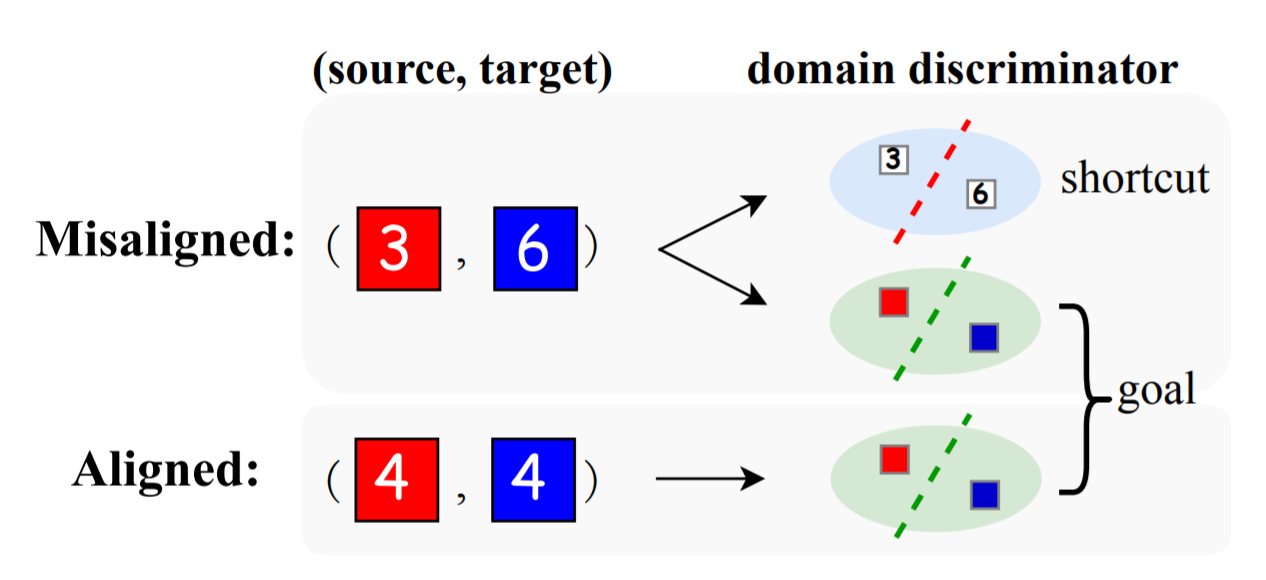
\includegraphics[scale=0.38]{Week07_shortcut.png}
                    \caption{Domain Discriminator Shortcut 解释}
                    \label{fig:shortcut}
                \end{figure}
            \subsubsection{Implicit Class-Conditioned Domain Alignment}

                \begin{figure}[ht]
                    \centering
                    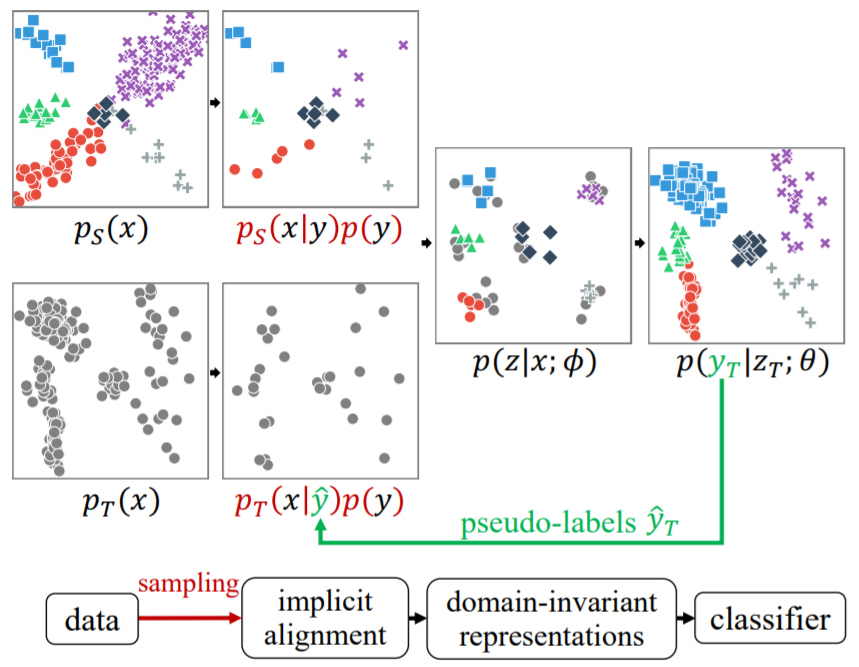
\includegraphics[scale=0.4]{Week07_implicit.png}
                    \caption{Implicit Alignment}
                    \label{fig:implicit}
                \end{figure}

                Implicit Class-Conditioned Domain Alignment 的过程如图 \ref{fig:implicit} 所示。
                将 source domain $p_S(x)$ 与 target domain $_T(x)$ 进行对齐,对于 $p_S(x)$,基于 alignment 分布 $p(y)$ 生成样本 $x \sim p_S(x|\hat{y})p(y)$ (如何生成?)。
                对于 $p_T(x)$,利用生成的伪标签 $\hat{y}_T$,使用相同的 $p(y)$ 生成 class aligned minibatch $x\sim p_T(x|\hat{y})p(y)$ (如何生成?)。
                然后使用对抗训练的方式从参数为 $\Phi$ 的特征提取器中获得与域无关 (domain-invariant) 的 representation $z$。
                最后分类器利用 $z$ 进行类预测。

                Class-aligned 样本的生成过程:

                首先使用分类器 $f_c(\dot;\theta)$ 生成 target domain 的伪标签,从 label space $\mathcal Y$ 中
                取样一个集合 $Y$ (其中 $p(y)$ 表示选取类别进行 align 的概率?)使得 source 和 target 共用同一个 $Y$,
                这个反过来使 class-misaligned divergence $\xi^{\overline{C}}(h, h')$ 最小化。
                接下来对于每个 $y_i \in Y$,分别为 source 和 target 取样一个 class-conditioned 样本,
                记为 $(X'_S, Y'_S)$ 和 $X'_T$。上面的操作等价于在表中寻找一个所有样本都属于 $y_i$ 的子集 $\mathcal B_i$,
                然后在 $\mathcal B_i$ 中进行随机取样。

                在得到 class aligned minibatch 后,进行无监督自适应的训练,重复这个过程直到模型收敛。

                论文采用了 Margin Disparity Discrepancy (MDD) 作为 domain divergence 的度量,其中 MDD 是一个基于分类器的域差异度量方法,
                其定义如下:

                $$
                    d_{f,\mathcal F}( S, T)=\sup_{f'\in\mathcal F}\Big{(}\text{disp}_{\mathcal{D}_T}(f',f)-\text{disp}_{\mathcal{D}_S}(f',f)\Big{)}
                $$

                其中 $f$ 和 $f'$ 是两个独立的 scoring 函数(分类器),用于预测 class 的概率,
                $\text{disp}(f, f')$ 是一个测量 $f$ 和 $f'$ 打分差异的函数。域的差异则通过两个域的 disparity measure (disp函数)来体现。

                \begin{figure}[ht]
                    \centering
                    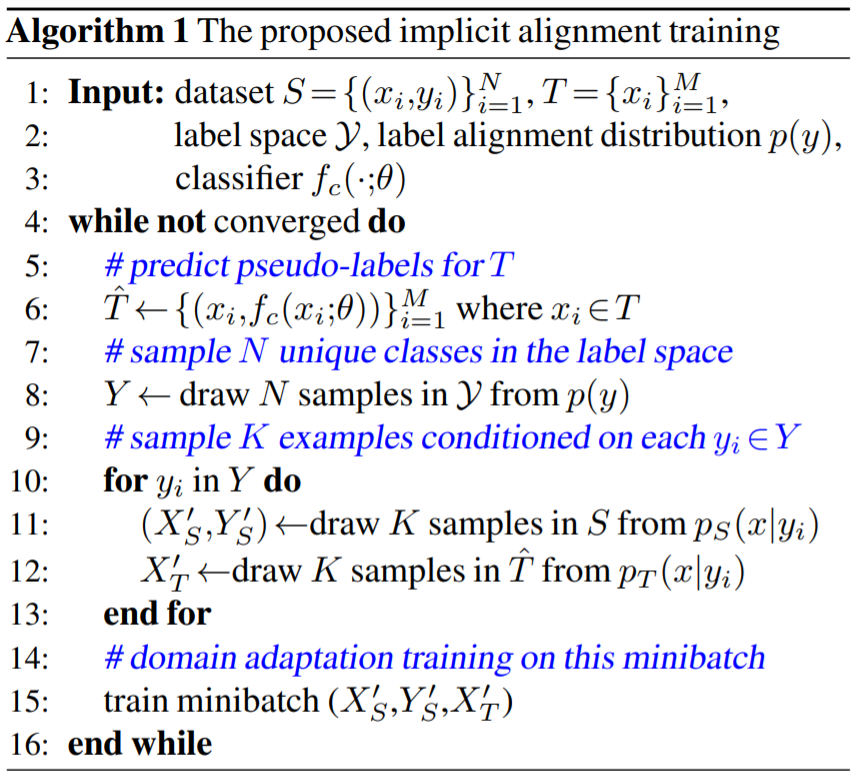
\includegraphics[scale=0.36]{Week07_train.png}
                    \caption{Implicit Alignment Training}
                    \label{fig:train}
                \end{figure}

                将 MDD 应用到 class-misaligned 的样本上,则有如下形式:

                $$
                    \hat{d}_{f,\mathcal F}( \mathcal{B}^{\overline{C}}_{S}, \mathcal{B}^{\overline{C}}_{T})=\sup_{f'\in\mathcal F}\Big{(}\sum_{\mathcal{B}^{\overline{C}}_{T}}\text{disp}(f',f)-\sum_{\mathcal{B}^{\overline{C}}_{S}}\text{disp}(f',f)\Big{)}
                $$

                由于 $\mathcal{B}^{\overline{C}}_{S}$ 和 $\mathcal{B}^{\overline{C}}_{T}$ 在 label space 上是不相交的,存在一个如下形式的 shortcut 函数:

                \begin{equation}
                    \text{disp}(f'(x),f(x))=\left\{
                    \begin{matrix}
                    0 & f_c(x)\in \overline{Y_{S}}\\ 
                    1 & f_c(x)\in \overline{Y_{T}}
                    \end{matrix}\right.
                \end{equation}

                这个 shortcut 函数会使得前面的 divergence 最大化(?)。
                由于伪标签存在问题,对于 misalignment 的影响很难评估,文中提出使用 masking 的方法更深入地对 class-misalignment 的影响进行评价,
                即对于两个 scoring 函数 $f$ 和 $f'$ 进行掩码(masking)操作:

                $$
                    \hat{d}_{f,\mathcal F}( \mathcal{B}_S, \mathcal{B}_T) =\\
                    \sup_{f'\in\mathcal F}\Big{(}\sum_{\mathcal{B}_T}\text{disp}(f'\odot\omega,f\odot\omega)-\sum_{\mathcal{B}_S}\text{disp}(f'\odot\omega,f\odot\omega)\Big{)}
                $$

                其中 $f\odot\omega$ 表示 element-wise 的乘法操作。Alignment mask $\omega$ 是一个 binary 向量,
                表示第 $i$ 个类是否在 sample 的类集 $Y$ 中(表示当前 minibatch 中想要进行 align 的类)。

                整个 Implicit Alignment 的训练过程如图 \ref{fig:train} 所示。

            \subsubsection{Experiment}
                使用的数据集为 Offic-31,Offic-Home 和 VisDA2017,其中 Office-Home 有三个版本:

                \begin{enumerate}
                    \item standard:原始数据集
                    \item balanced:原始数据集的子集,每个 class 中的 example 数量相同
                    \item RS-UT:两个 domain 都是 imbalance 的,并且 source 中数据多的 class 是 target 中数据少的 class
                \end{enumerate}

                模型采用在 ImageNet 上预训练的 ResNet-50,实验的结果如图 \ref{fig:RS-UT}, \ref{fig:Office-31}, \ref{fig:Office-Home}, \ref{fig:VisDA} 所示。

                \begin{figure}[ht]
                    \centering
                    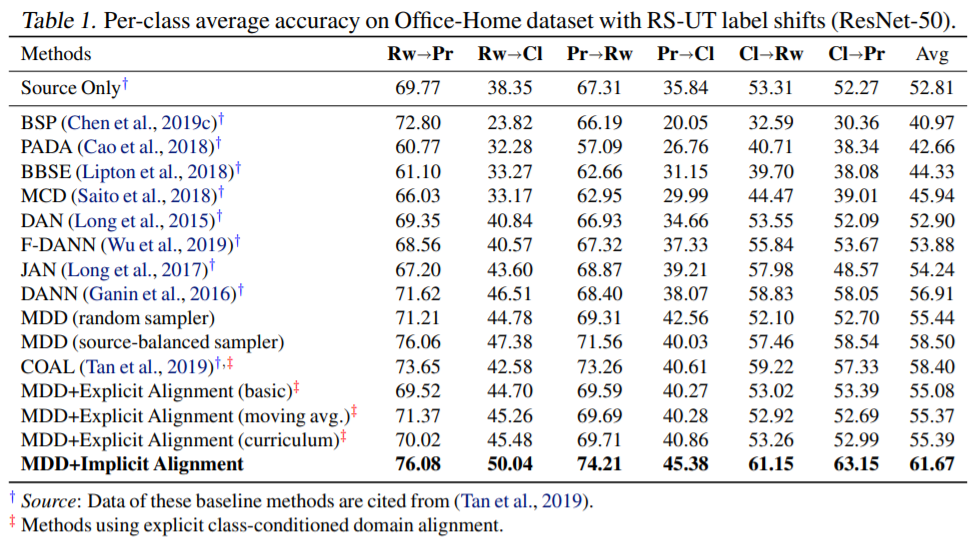
\includegraphics[scale=0.4]{Week07_RS-UT.png}
                    \caption{Office-Home RS-UT 实验结果}
                    \label{fig:RS-UT}
                \end{figure}

                \begin{figure}[ht]
                    \centering
                    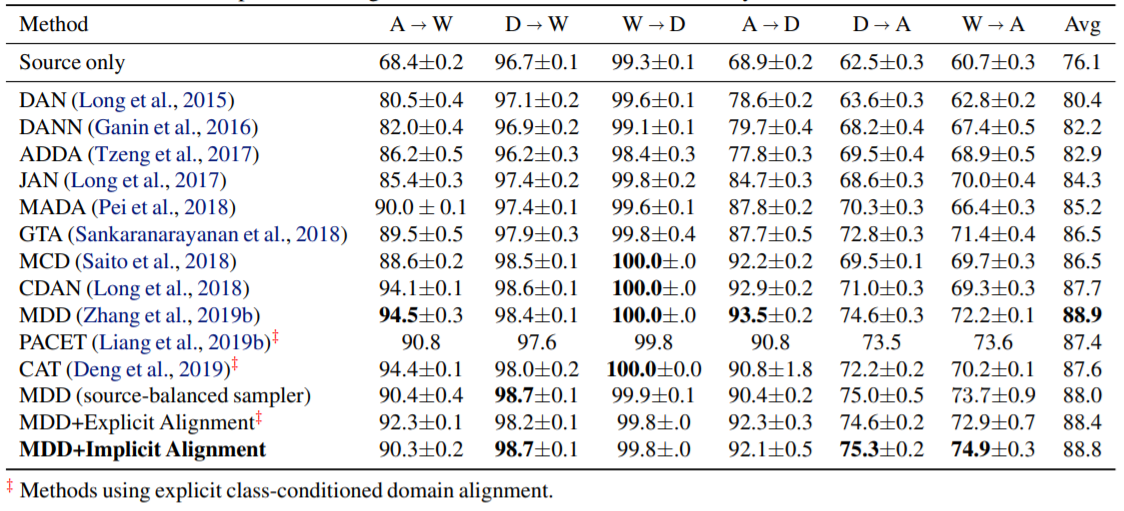
\includegraphics[scale=0.4]{Week07_Office-31.png}
                    \caption{Office-31 实验结果}
                    \label{fig:Office-31}
                \end{figure}

                \begin{figure}[ht]
                    \centering
                    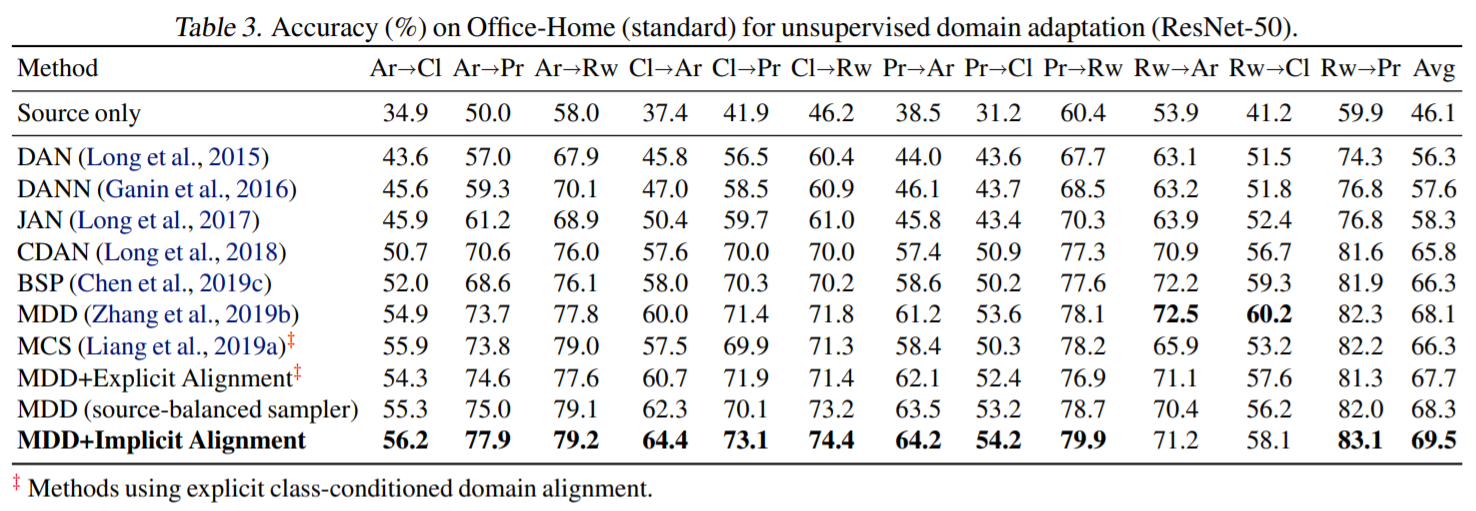
\includegraphics[scale=0.3]{Week07_Office-Home.png}
                    \caption{标准 Office-Home 实验结果}
                    \label{fig:Office-Home}
                \end{figure}

                \begin{figure}[ht]
                    \centering
                    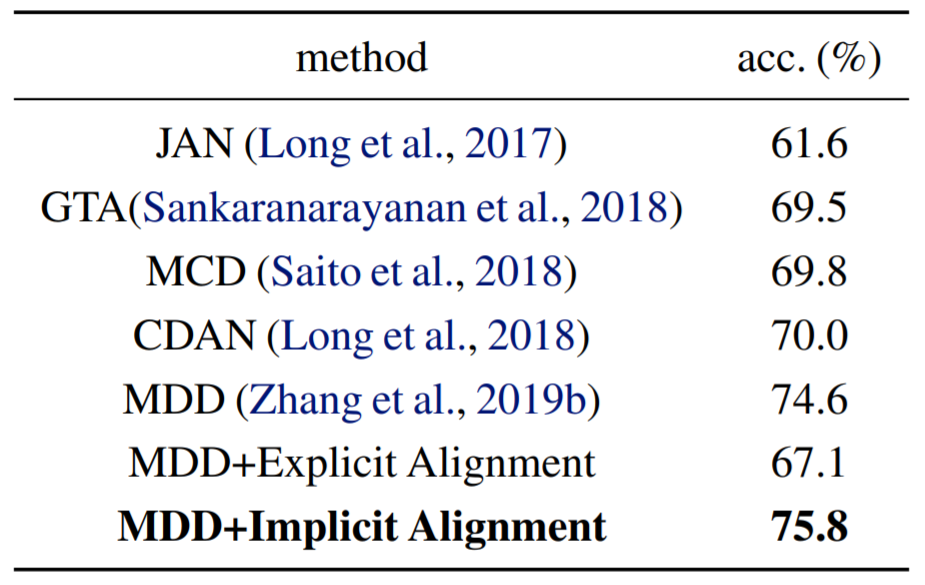
\includegraphics[scale=0.4]{Week07_VisDA.png}
                    \caption{VisDA2017 实验结果}
                    \label{fig:VisDA}
                \end{figure}

                可以看到,MDD+implicit alignment 的方法在效果上的提升是非常显著的,
                这也说明 implicit 的方法确实比 explicit 的方法效果更好。
            \subsubsection{小结}
                这篇文章解决的其实是 source 和 target 之间的 class 存在 shift 的问题,也是我之前想要解决的问题。
                这个问题在 MSDA 的任务中也是存在的,可以从两个角度去考虑解决方法,
                一个是建立多个 source 和 target 之间的 shortcut 函数,将原本的二分类任务推广;
                另一个是对每个 source 分别与 target 进行 shortcut 的计算,然后再整合。
    \section{启发}
        \begin{enumerate}
            \item 可以考虑论文中给出的方法,将情形推广到多源的情况,分析多源情况下的 implicit domain alignment
            \item 文中在处理 misalignment 问题时,提到了一个 masking 的操作,可以使得每个 minibatch 中对不同的 class 进行处理
        \end{enumerate}
    \section{疑问/困难}
        \begin{enumerate}
            \item 文中给出的 implicit domain alignment 是基于单源领域自适应的,在多源情况下,不同域之间的关系并不能直接用一条 shortcut 画出来,
                如果要设计多个 source 与 target 之间的 shortcut 函数,其形式不再是简单的 binary。如果采用每个 source 分别与 target 构成 shortcut 函数再组合的方法,
                则每个 source 与 target 的组合之间都存在类差异。
            \item 使用 masking 的方式只能对确定的类进行操作,当 target 存在未知类时,并不能用人为设定 masking 的方式来对特定类进行 alignment。
            \item 这篇文章的 domain alignment 主要关注点在 class 上,如果是在 feature map 上进行 alignment,由于重叠和不重叠的 feature 是未知的,
            也就无法选择交集和差集进行 shortcut 函数的设计(也许可以放在 PAL 筛选过后进行进一步训练?)。
        \end{enumerate}
\end{document}
